\documentclass{article}
\usepackage{tikz}
\usetikzlibrary{mindmap, trees}
\begin{document}

\begin{figure}[h]
\centering
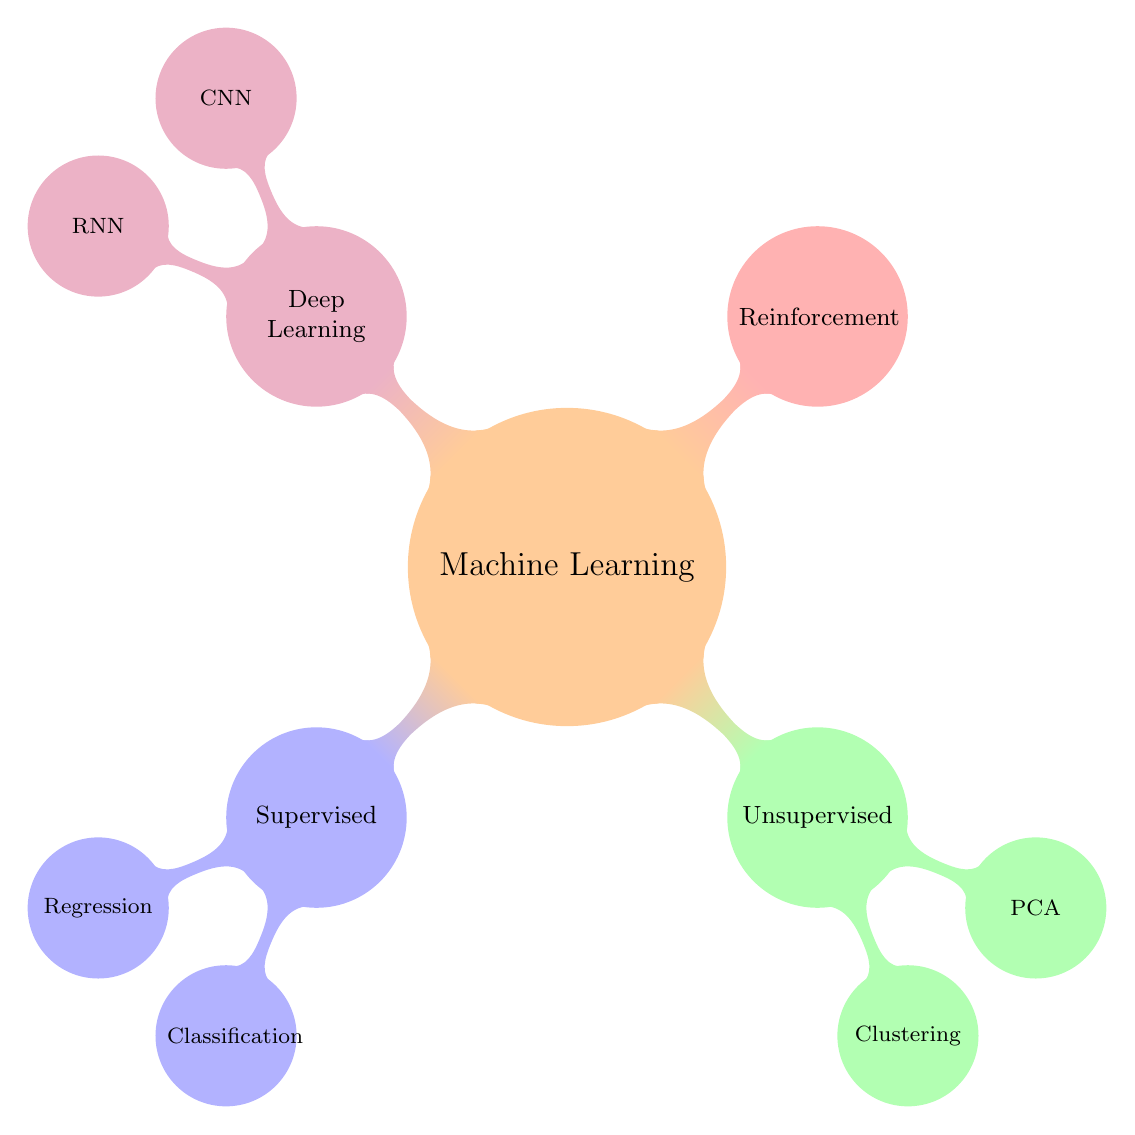
\begin{tikzpicture}[mindmap, grow cyclic, every node/.style=concept, concept color=orange!40,
  level 1/.append style={level distance=4.5cm, sibling angle=90},
  level 2/.append style={level distance=3cm, sibling angle=45}]
\node{Machine Learning}
  child[concept color=blue!30] { node {Supervised}
    child { node {Regression}}
    child { node {Classification}}
  }
  child[concept color=green!30] { node {Unsupervised}
    child { node {Clustering}}
    child { node {PCA}}
  }
  child[concept color=red!30] { node {Reinforcement}}
  child[concept color=purple!30] { node {Deep Learning}
    child { node {CNN}}
    child { node {RNN}}
  };
\end{tikzpicture}
\caption{A mind map of machine learning.}
\end{figure}

\end{document}
